\begin{wrapfigure}[10]{r}[0pt]{100mm}
	\centering
    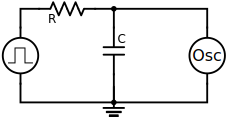
\includegraphics[width=80mm]{schema.pdf}
    \caption{Schema del circuito utilizzato.}
    \label{fig:circuito}
\end{wrapfigure}


\section{Strumenti}

%\begin{multicols}{2}
$\bullet \quad$Oscilloscopio \\
$\bullet \quad$Cablaggio\\
$\bullet \quad$Decadi di resistenze e capacità\\
$\bullet \quad$Generatore di forme d'onda\\
$\bullet \quad$Multimetro digitale\\
$\bullet \quad$Breadboard (basetta sperimentale)\\
%\columnbreak
%\begin{figure}[h!]
%	\centering
%	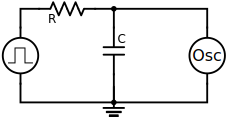
\includegraphics[width=\textwidth]{schema.pdf}
%    \caption{Schema del circuito utilizzato.}
%    \label{fig:circuito}
%\end{figure}

%\end{multicols}
\hspace{2pt}\\

\section{Preparazione circuito}

Inizialmente abbiamo collegato il generatore di forme d'onda all'oscilloscopio (uscita 1) per ottenere la forma d'onda con cui confrontare quella ricavata dall'analisi del circuito.
In seguito è stato preparato il circuito, inizialmente come semplice circuito chiuso composto di generatore di ddp variabile (generatore di forme d'onda), resistenza e condensatore in serie. Successivamente abbiamo collegato in parallelo al condensatore l'oscilloscopio (uscita 2).

La resistenza e il condensatore usati sono in realtà \textit{decadi di resistenze} e \textit{decadi di condensatori}. Questo tipo di resistenze e condensatore sono formati da una scatola contenente diverse resistenze in serie o condensatori in parallelo e il circuito che li connette può essere modificato tramite diverse manopole permettendo di cambiare la resistenza totale o la capacità totale del circuito.

\section{Parametri oscilloscopio e generatore di forme d'onda}

Una volta collegato il circuito all'oscilloscopio abbiamo dovuto tarare le scale con cui esso leggeva i dati in input e alcuni parametri con cui il generatore d'onda immetteva nel circuito la sua differenza di potenziale. Lo studio della costante di tempo $\tau$ infatti richiede che il condensatore si carichi (o scarichi) completamente.
Innanzitutto per comodità di calcolo abbiamo scelto di produrre un'onda quadra con ampiezza di 1.000 Vpp\footnote{Vpp = volt picco picco} e abbiamo settato un offset di $0.500\si{\volt}$ (?) in modo da ottenere un'onda con $V_{min}=0\,\si{\volt}$ e $V_{min}=1\,\si{\volt}$